\documentclass[12pt,paper=a4]{report}
\usepackage{fontspec}
\usepackage{xunicode}
\usepackage{xltxtra}
\usepackage{polyglossia}
\setdefaultlanguage{latvian}
\usepackage{fixlatvian}
\usepackage{caption}
\setotherlanguages{english,russian,french}
\setmainfont[Mapping=tex-text]{Times New Roman}%{LMRoman10}
% Fonts krievu valodai, kurā ir arī krievu valodas burti
\newfontfamily\russianfont{Times New Roman}
% Šos fontus tālāk izmantos chapter virsrakstos un url'os (lai būtu kirilicas burti)
\newfontfamily\sffamily{Verdana}
\captionsetup{justification=centering}
\usepackage{setspace}

% lai varam normāli rakstīt apakšvītras
\usepackage{underscore}
% Lai varam iekļaut attēlus
\usepackage{graphicx}
% Kurā vietā tiks meklēti attēli - relatīvais ceļs attiecībā pret dokumentu
\graphicspath{{./PNG/}{./images/internet/}{./images/self-generated/}}
% Ar šiem PDF'ā būs saliktas saites un tām va uzlikt krāsu
\usepackage{hyperref}
\hypersetup{ colorlinks, citecolor=black, filecolor=black,linkcolor=black,urlcolor=black }

\usepackage{amsmath}
\usepackage{amsfonts}
\usepackage{lipsum} %Lai ģenerētu nejaušus tekstus...
\usepackage{listingsutf8}
\usepackage{xcolor}

%\usepackage{inconsolata}
\lstset{
    language=bash, %% Troque para PHP, C, Java, etc... bash é o padrão
    basicstyle=\ttfamily\small,
    numberstyle=\footnotesize,
    numbers=left,
    backgroundcolor=\color{gray!10},
    frame=single,
    tabsize=2,
    rulecolor=\color{black!30},
    title=\lstname,
    escapeinside={\%*}{*)},
    breaklines=true,
    breakatwhitespace=true,
    framextopmargin=2pt,
    framexbottommargin=2pt,
    extendedchars=false,
    inputencoding=utf8
}


%% Mainīt chapteru izskatu - centrēts un definētais sffamily fonts (skatīt augstāk)
\usepackage{titlesec}
\titleformat{\chapter}{\huge\centering\sffamily}{\thechapter}{1pc}{}

%% Pārdēvējam ``Literatūra`` par ``Izmantotās literatūras un avotu saraksts''.
\addto\captionslatvian{
\renewcommand\bibname{Izmantotās literatūras un avotu saraksts}
}

%% Atraitņrindiņas un bāreņrindiņas ( widow orphan) vadība
\clubpenalty10000
\widowpenalty10000

%% Visādas atkāpes - 1" (2.54 cm) atkāpe jau ir pēc noklusējuma, šeit tikai korekcijas
%\setlength{\parskip}{1line}
\setlength{\topmargin}{0cm}
\setlength{\headheight}{0in}
\setlength{\headsep}{0in}
\setlength{\textheight}{22.7cm}
\setlength{\textwidth}{15cm}
\setlength{\oddsidemargin}{0.5in}
\setlength{\evensidemargin}{0.5in}
%\setlength{\parindent}{0.25in}
%\setlength{\parskip}{0.25in}

%% uzliekam atkāpes arī nodaļu 1. rindkopas 1. rindai
\usepackage{indentfirst}

%Pārnesumiem - ļauj tiasīt lielākas starpas
\hyphenpenalty=5000

%% Nodaļu un apakšnodaļu numerācija tagad to veic fixlatvian package
%\def\thechapter      {\arabic{chapter}.}
%\def\thesection      {\ifx\chapter\undefined{\arabic{section}.}\else  %{\thechapter\arabic{section}.}\fi}
%\def\thesubsection   {\thesection\arabic{subsection}.}
%\def\thesubsubsection{\thesubsection\arabic{subsubsection}.}
%\def\theparagraph    {\thesubsubsection\arabic{paragraph}.}
%\def\thesubparagraph {\theparagraph\arabic{subparagraph}.}

%% Pakotne lai saliktu automātisku figūru skaitīšanu
\usepackage{totcount}

\newcounter{nofappendices}
\setcounter{nofappendices}{0}
\regtotcounter{nofappendices}

\newtotcounter{fignum}
\def\oldfigure{} \let\oldfigure=\figure
\def\figure{\stepcounter{fignum}\oldfigure}

%defineejam atsauču skaitītāju
\newtotcounter{citnum}
\def\oldbibitem{} \let\oldbibitem=\bibitem
\def\bibitem{\stepcounter{citnum}\oldbibitem}

%% Attēlu numerācija
%\renewcommand{\thefigure}{\arabic{chapter}.\arabic{figure}.}

%% Sarakstam visus mainīgos
%% Mainīgie titullapai, defAutors tiek izmantots arī galvojumā
\def\defAutors{Edgars Skore}
\def\defAugstskola{Ventspils Augstskola}{\fontfamily{russianfont}
\def\defFakultate{Informācijas tehnoloģiju fakultāte}
\def\defSProgrammas{dabas zinātņu maģistra studiju programmas\\
	      datorzinātnēs}
\def\defStudents{2. kursa students \\
	      \defAutors}
\def\defMatrikulasNr{16080002}
\def\defDarbaNosaukums{Cilvēku plūsmas analīze, pielietojot konvolūcijas tīklus}
\def\defDarbaNosaukumsEN{Human flow analysis using Convolutional Neural Networks}
\def\defDarbaNosaukumsFR{La grande question sur la vie, l'univers et le reste}
\def\defDarbaNosaukumsLV{Pagātnes, tagadnes un nākotnes aspekti atbildei uz galveno jautājumu}
\def\defDarbaNosaukumsRU{Ответ на главный вопрос жизни, вселенной и всего такого}
\def\defDarbaVeids{Maģistra darbs}
\def\defFakultatesDekans{doc.  Dr.phys. M.~Ēlerts}
\def\defZinVaditajs{Dr.sc.comp. Gundars Bergmanis-Korāts}
\def\defGads{2018}
 %šeit pārdefinējam savus mainīgos (atstāju iepriekšējās rindas, lai varētu redzēt pārdefinēšanu)

%% pievienota anotācijas noformēšana
%\usepackage{etoolbox}% http://ctan.org/pkg/etoolbox
%\makeatletter
%\patchcmd{\@makechapterhead}{\vspace*{50\p@}}{}{}{}% Removes space above \chapter head
%\setafterchapterskip{1sp}
%defineejam anotaacijas lapas, lai vareetu vienkaarshaak taas izmantot
\def\abstract{
  %\section*{\begin{center} \abstractname \end{center}} % start chapter

\vspace*{-4\baselineskip}
	\chapter*{\begin{center} \abstractname \end{center} } % start chapter
	\vspace*{-2.5\baselineskip}
  \addcontentsline{toc}{chapter}{\abstractname} % table of contents line
  \markboth{\MakeUppercase{\abstractname}}{} % header mark
}
\def\endabstract{}%\clearpage

%% Beidzot sākam rakstīt dokumentu
\begin{document}

%% Vislabāk nodaļas rakstīt kā atseviškus failus, kurus iekļauj ar input (.tex paplašinājums pats tiek pielikts klāt)
% \input{src/mag-titullapa} %% visu titullapu ērtāk ir turēt datnē mag-titullapa.tex, bet te mēs tomēr visu rakstīsim vienā vietā:

%%%% Titullapas sākums
%%%% Titullapas sākums
\begin{titlepage}
\begin{center}
\textsc{
\defAugstskola\\
\defFakultate}\\
\vspace{2em}
\textbf{\defDarbaVeids}\\
\vspace{2em}
{\LARGE \textbf{\defDarbaNosaukums}}\\
\vspace{2em}
\begin{tabular}{@{}r@{}l@{}}
\parbox[c]{0.4\textwidth}{Autors:}&
\parbox[t]{0.6\textwidth}{
\defAugstskola s\\
\defFakultate s\\
\defSProgrammas\\
\defStudents \\
Matrikulas~Nr. \defMatrikulasNr\vspace{0.7em}\\
\mbox{}\hrulefill\vspace{-0.4em}\\
{\scriptsize(paraksts)}\vspace{2em}} \\
\parbox[c]{0.4\textwidth}{Fakultātes dekāns:}&
\parbox[t]{0.6\textwidth}{
\defFakultatesDekans\vspace{.7em}\\
\mbox{}\hrulefill\vspace{-0.4em}\\
{\scriptsize(paraksts)}\vspace{2em}} \\
\parbox[c]{0.4\textwidth}{Zinātniskais vadītājs:}&
\parbox[t]{0.6\textwidth}{
\defZinVaditajs\vspace{.7em}\\
\mbox{}\hrulefill\vspace{-0.4em}\\
{\scriptsize(paraksts)}\vspace{2em}} \\
\parbox[c]{0.4\textwidth}{Recenzents:} & \vspace{.7em}\\
\multicolumn{2}{@{}c@{}}{
\mbox{}\hrulefill
}\vspace{-0.4em}\\
\multicolumn{2}{@{}l@{}}{
{\scriptsize(Ieņemamais amats, zinātn. nosaukums,
vārds, uzvārds)}
}\vspace{.7em}\\
&\mbox{}\hrulefill\vspace{-0.4em}\\
&{\scriptsize(paraksts)}\\
\end{tabular}
\vfill
Ventspils, \defGads
\end{center}
\end{titlepage} %pievienota titullapa, kura izveidota atsevišķā failā
%%%% Titullapas beigas

%%%% Satura rādītājs
\tableofcontents

%%%% 1.5 līiniju atstarpe starp rindām
\onehalfspace

{
	\selectlanguage{latvian}
	\begin{abstract}
		
		\begin{tabular}{@{}r@{}l@{}}
			\parbox[c]{0.3\textwidth}{\textbf{The title:}}&
			\parbox[t]{0.65\textwidth}{\defDarbaNosaukumsEN} \\
			\parbox[c]{0.3\textwidth}{\textbf{Autors:}}&
			\parbox[t]{0.65\textwidth}{\defAutors} \\
			\parbox[c]{0.3\textwidth}{\textbf{Academic Advisor:}}&
			\parbox[t]{0.65\textwidth}{\defZinVaditajs} \\
			\parbox[c]{0.3\textwidth}{\textbf{The volume of the work:}}&
			\parbox[t]{0.65\textwidth}{\textcolor{black}{\pageref{LastPage}} pages, XX~tables,  \total{fignum}~images, XX~equations, \total{citnum}~literature sources, \total{nofappendices}~appendices} \\
			\parbox[c]{0.3\textwidth}{\textbf{Keywords:}}&
			\parbox[t]{0.65\textwidth}{ Life, Universe, Questions, Philosophy} \\
			&\\
		\end{tabular}
		%\total{nofimages} % ja nu gadiijumaa vajag custom counter
		
		In the first novel and radio series, a group of hyper-intelligent pan-dimensional beings demand to learn the \textbf{Answer to the Ultimate Question of Life} from the supercomputer, Deep Thought, specially built for this purpose. It takes Deep Thought 7½ million years to compute and check the answer, which turns out to be\textbf{ 42}.  Unfortunately, The Ultimate Question itself is unknown.\cite{wiki-en}
		
	\end{abstract}
}

%%%% 1.5 līiniju atstarpe starp rindām
\onehalfspace
{
\selectlanguage{english}
\begin{abstract}

\begin{tabular}{@{}r@{}l@{}}
\parbox[c]{0.3\textwidth}{\textbf{The title:}}&
\parbox[t]{0.65\textwidth}{\defDarbaNosaukumsEN} \\
\parbox[c]{0.3\textwidth}{\textbf{Author:}}&
\parbox[t]{0.65\textwidth}{\defAutors} \\
\parbox[c]{0.3\textwidth}{\textbf{Academic Advisor:}}&
\parbox[t]{0.65\textwidth}{\defZinVaditajs} \\
\parbox[c]{0.3\textwidth}{\textbf{The volume of the work:}}&
\parbox[t]{0.65\textwidth}{\textcolor{black}{\pageref{LastPage}} pages, XX~tables,  \total{fignum}~images, XX~equations, \total{citnum}~literature sources, \total{nofappendices}~appendices} \\
\parbox[c]{0.3\textwidth}{\textbf{Keywords:}}&
\parbox[t]{0.65\textwidth}{ Life, Universe, Questions, Philosophy} \\
&\\
\end{tabular}
%\total{nofimages} % ja nu gadiijumaa vajag custom counter

In the first novel and radio series, a group of hyper-intelligent pan-dimensional beings demand to learn the \textbf{Answer to the Ultimate Question of Life} from the supercomputer, Deep Thought, specially built for this purpose. It takes Deep Thought 7½ million years to compute and check the answer, which turns out to be\textbf{ 42}.  Unfortunat  ely, The Ultimate Question itself is unknown.\cite{wiki-en}

\end{abstract}
}

%%%% Nodaļa bez numerācijas
\chapter*{Izmantotie saīsinājumi un termini}
\addcontentsline{toc}{chapter}{Izmantotie saīsinājumi un termini}

%%%  Sākas nodaļas
\chapter{Ievads}
Ievadā ir jāietver:

\begin{itemize}
\item temata aktualitātes pamatojums;
\item darba mērķis;
\item darba mērķa sasniegšanai veicamo uzdevumu formulējums;
\item izmantojamo pētīšanas metožu un paņēmienu uzskaitījums;
\item literatūras un avotu grupu uzskaitījums (piemēram, speciālā ekonomiskā literatūra, valsts statistikas dati, nepublicētie materiāli no uzņēmuma arhīva u.c.);
\item darba struktūras apraksts;
\item pētījuma temata un perioda norobežojums (ja tas nepieciešams).
\end{itemize}

Mašīnmācīšanās algoritmi ir kļuvuši par neatņemamu sastāvdaļu programmatūras izstrādātājiem un kompānijām, kas savas aplikācijas grib padarīt "gudras". Lai arī cik, mūsdienās, šis jēdziens ir kļuvis populārs, oficiāla mašīnmācīšanās definīcija nav noteikta. Visvienkāršākais mašīnmācīšanās pielietojums ir apstrādāt datus, mācīties no tiem un no iegūtajiem rezultātiem pieņemt lēmumus vai veikt minējumus reālās pasaules problēmu risināšanai. Tā vietā, lai manuāli veidotu programmatūras risinājumus, kas veic kādu uzdevumu, tiek apmācīti datori vai citas ierīces, izmantojot lielus datu apjomus. 
\section{Mašīnmācīšanās pamatjēdziens}
Pasaulē ir daudz un dažādi mašīnmācīšanās algoritmi un katru dienu tiek publicēti simtiem jaunu algoritmu. Tos var sagrupēt pēc apmācības veida (vadītā apmācība (\textit{supervised learning}), nevadītā apmācība (\textit{unsupervised learning}), pusvadītā apmācība (\textit{semi-supervised learning})) kā arī pēc formas vai funkcijas līdzībām (klasifikācija, regresija, lēmumu koki (\textit{decision trees}), klasterēšana (\textit{clustering}), dziļā mašīnmācīšanās (\textit{deep learning})). Neatkarīgi no apmācības veida vai pielietojuma, visas mašīnmācīšanās algoritmu kombinācijas sastāv no klasifikatoriem (atbalsta vektora mašīna, lēmuma koki, neironu tīkli), vērtēšanas funkcijām (varbūtības funkcijas, robežfunkcijas, izmaksu funkcija) un optimizācijas funkcijām (mantkārīgā meklēšana, nepārtrauktās optimizācijas metodes (\textit{continuous optimization})). Izmantojot šīs sastāvdaļas, mašīnmācīšanās algoritmu pamata mērķis ir būt spējīgam funkcionēt ne tikai ar apmācībā piedāvātajiem datiem, bet arī spēt darboties ar datiem, ar kuriem algoritms nav saskāries. Atkarībā no veicamā uzdevuma, ir dažādi veidi kā panākt, lai datori vai jebkura cita ierīce mācās, sākot ar visparastākajiem lēmumu kokiem, beidzot ar ģenētiskajiem algoritmiem un mākslīgajiem neironu tīkliem. 


\newpage
\section{Datorredze}
Datorredze (no angļu val. \textit{computer vision}) ir datorzinātņu nozare, kuras mērķis ir ļaut datoriem redzēt un veikt tādus pašus uzdevumus kā cilvēki veiktu ar acīm un darīt to tikpat efektīvi. Redzes nodrošināšana datoriem nozīmē dot tiem spēju identificēt un apstrādāt attēlus līdzīgi kā to spēj darīt cilvēki. Tas ir kā nodot cilvēku inteliģenci un instinktus datoram. Datorredzes sistēmas parasti iedala trīs komponentēs:
\begin{itemize}
	\item Attēla iegūšana;
	\item Attēla apstrāde;
	\item Attēla analīze;
\end{itemize}
Līdzīgi kā cilvēku pasaules izpratne balstās uz spēju pieņemt lēmumus ņemot vērā redzēto, piedāvājot datoriem šādu vizuālu izpratni, tiem būtu iespējams pieņemt patstāvīgus lēmumus.

\begin{figure}[h]%
	\centering
	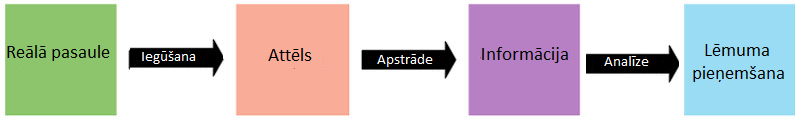
\includegraphics[height=2cm]{images/computervision1.png} %
	\caption{Datorredzes pamatprincips}%
	\label{fig:example}%
\end{figure}

Attēlu iegūšana ir process kurā reālās pasaules notikumi tiek pārveidoti bināros datos, kurus interpretē kā digitālus attēlus vai kā daļu no video fragmenta. 

Attēlu apstrāde ir iegūto attēlu zema līmeņa apstrāde. Pirmajā solī iegūtajiem binārajiem datiem pielieto algoritmus, kas norāda uz attēla daļām, kas satur zema līmeņa informāciju. Šādu informāciju var izšķirt pēc jebkādiem ģeometriskiem elementiem, kas sastāda attēlu, piemēram, punkti attēlā, attēla malas vai segmenti. Zema līmeņa attēlu apstrādes algoritmi ir malu detektēšana, segmentācijas algoritmi, klasifikācija, īpašību detektēšana.
\begin{figure}[h]%
	\centering
	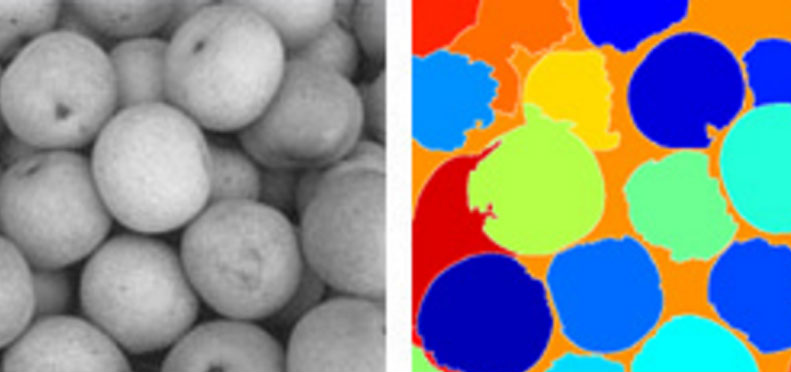
\includegraphics[height=3cm]{images/computervision2.png} %
	\caption{Ābolu segmentācija attēlā \cite{compv1}}%
	\label{fig:example}%
\end{figure} 

Pēdējā datorredzes sistēmu komponente ir attēlu analīzes solis, kurā notiks attēla analīze un pēc šī soļa datorredzes sistēmai būs iespējams pieņemt lēmumu un izvadē to atgriezt. Attēlu analīzes solī tiek pielietoti augsta līmeņa algoritmi, ņemot vērā gan attēla apstrādes solī iegūto zema līmeņa informāciju, gan pašu attēlu. Piemēri kur var izmantot šādu augsta līmeņa attēlu analīzi ir trīsdimensiju ainu atveidošana, objektu atpazīšana, objektu sekošana, cilvēku plūsmas analīze.
\begin{figure}[h]%
	\centering
	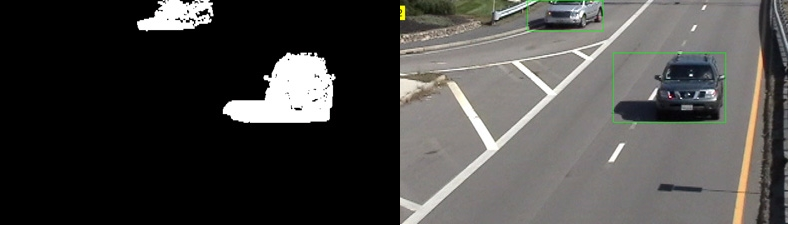
\includegraphics[height=4cm]{images/computervision3.png} %
	\caption{Objektu detektēšana pēc segmentācijas pielietošanas \cite{compv2}}%
	\label{fig:example}%
\end{figure} 

Izstrādājot datorredzes sistēmas, pētnieki saskaras ar dažādām problēmām un izaicinājumiem. Parasti šīs problēmas ir atkarīgas no datu kvalitātes, sistēmas pielietojuma un apkārtējās pasaules ietekmes uz datiem un aparatūru. Datorredzes pētnieki izstrādā risinājumus, lai padarītu datorredzes algoritmus stabilākus un efektīvākus sarežģītos uzstādījumos: nekvalitatīvi vai trokšņaini dati, reālā laika apstrāde un ierobežota skaitļošanas jauda. Mūsdienās, lai risinātu šīs problēmas, tiek savienoti mašīnmācīšanās risinājumi ar datorredzes risinājumiem.

Klasiskie datorredzes algoritmi ir smalki pētīti un optimizēti, lai iegūtu labāko veiktspēju un lai tie efektīvi izmantotu datora skaitļošanas resursus, kamēr mašīnmācīšanās algoritmi piedāvā precīzākus un vispusīgākus risinājumus, taču prasa lielus skaitļošanas resursus. Ņemot vērā iepriekš minēto, mūsdienu pētījumos ir populāri risinājumi, kas apvieno standarta datorredzes algoritmus un mašīnmācīšanās risinājumus. Labs piemērs abu šo nozaru apvienošanā ir kustīgu objektu meklēšana video fragmentos. Lai iegūtu augstāku precizitāti un taupītu skaitļošanas resursus ir iespējams attēla apstrādi veikt ar datorredzes algoritmiem un attēla analīzi (klasifikāciju, lokalizāciju, sekošanu) veikt ar neironu tīkliem.



 %% Ērtāk visu ir rakstīt atsevišķos failos - ievads.tex un tad tos iekļaut ar input komandu

\chapter{Literatūras apskats}
Ir aprakstītas vairākas metodes, lai veiktu cilvēku plūsmu analīzi attēlos un video fragmentos \cite{brostow2006unsupervised,chen2013cumulative,ge2009marked,chen2015person,lempitsky2010learning}. Vispārīgi, pirmie pētījumi tika vērsti uz detektēšanas veida izvēli un vai problēmu var risināt izmantojot segmentācijas metodes \cite{tu2008unified}. Šīs metodes nelabvēlīgi ietekmēja objektu nostāšanās vienam aiz otra, objektu pazušana un nekārtīgs (pārblīvēts TODO pārbaudīt tulkojumu (high clutter background)) fons attēlos. Jaunākos risinājumus var vispārīgi sadalīt trīs kategorijās: risinājumi, kas balstīti uz regresiju, risinājumi, kas balstīti uz pūļa blīvuma novērtējumu un risinājumi, kas balstīti uz konvolūcijas neironu tīkliem. 

\subsubsection{Risinājumi, kas balstīti uz regresiju}
Lai novērstu objektu paslēpšanos attēlā un pārblīvēta fona problēmas, pētnieki mēģināja skaitīt cilvēkus izmantojot regresiju. Parasti, regresija šādos risinājumos tiek veikta starp dažādām attēla īpašībām un objektu skaitu. Šāds risinājums sadala attēlu vairākos mazākos attēlos un katram šim mazajam attēlam tiek veikta aptuvenā skaita noteikšana izmantojot segmentācijas metodes. Lai noteiktu kopējo cilvēku skaitu attēlā, ir jāsaskaita katra mazā attēla aptuvenie novērtējumi. Lai apmācītu šādu sistēmu, pirmais no attēla apstrādes posmiem ir atmest attēla fonu un veikt \textit{ground-truth} novērtējumu, kas nozīmē, ka tiek manuāli izskaitīts cilvēku skaits katrā sadalītajā attēlā  \cite{chan2009bayesian,ryan2009crowd,chen2012feature}.

Šāda pieeja tika izveidota, pieņemot, ka dotajai cilvēku skaitīšanas sistēmai būtu vieglāk novērtēt cilvēku daudzumu katrā grupā atsevišķi, nevis novērtēt cilvēku daudzumu visam pūlim vienlaikus. Pieņemot, ka attēlā ir pūlis ar 20 cilvēkiem, šo pūli var sadalīt divās lielās grupās vai arī desmit pāros. Ņemot šādu attēlu vispārīgi, šāds pūļa sadalījums var nebūt tik skaidri novērtējams, jo attēlam vispārīgi būtu daudz vairāk atšķirīgu īpašību. Eksistējošas metodes, kas izmanto visu attēlu no attēla iegūst daudz vairāk īpašību, kas nozīmē, ka ir nepieciešami vairāk apmācības datu \cite{chan2008privacy}. Pētot citus rakstus var secināt, ka regresijas metodes parasti sastāv no divām lielām komponentēm: zema līmeņa īpašību iegūšanas un regresijas modeļa implementēšanas \cite{xiong2017spatiotemporal}. 

\subsubsection{Risinājumi, kas balstīti uz pūļa blīvuma novērtējumu}
Lai gan pūļu skaitīšanas risinājumi, kas balstīti uz regresiju veiksmīgi tika galā ar objektu pārklāšanās un pārblīvētā fona problēmām, tika palaista garām svarīga telpiska informācija, jo regresija tika izmantota uz lokālajām īpašībām (katra sadalītā attēla īpašībām atsevišķi). Pētījumā \cite{lempitsky2010learning} tiek piedāvāts jauns veids kā iemācīties lineāras attiecības starp sadalīto attēlu īpašībām un attiecīgās objektu blīvuma kartes izmantojot regresiju. Novērojot, ka iemācīties lineāras attiecības ir sarežģīts uzdevums, tika izveidots risinājums, kas piedāvā iemācīties nelineāras attiecības starp sadalīto attēlu īpašībām un objektu blīvuma kartēm izmantojot nejaušo mežu ietvaru (no angļu val. \textit{random forest framework}) \cite{pham2015count}. Vairāki mūsdienu risinājumi piedāvā metodes, kas balstās uz blīvuma karšu regresiju \cite{wang2016fast,xia2016block}. 

\subsubsection{Risinājumi, kas balstīti uz konvolūcijas neironu tīkliem}
Tā kā mūsdienās klasifikācijā un atpazīšanas uzdevumu risināšanā ļoti veiksmīgi darbojas uz konvolūcijas neironu tīkliem balstītas metodes. Pētnieki ir izveidojuši CNN, ar mērķi veikt pūļa skaitīšanu un blīvuma novērtējumu \cite{wang2015deep,shang2016end,walach2016learning}. Pretēji jau eksistējošajām metodēm, kas pūļa skaitu novērtē izmantojot attēla sadalīšanas metodes, Šangs \cite{shang2016end} piedāvā metodi, kas veic novērtējumu izmantojot CNN. Šī metode novērtējumu veic paralēli skaitot cilvēkus gan globālajā kontekstā, gan lokālajā kontekstā. Žangs \cite{zhang2016single} piedāvāja daudz-kolonnu arhitektūru, kas izgūst īpašības dažādos mērogos. Līdzīgi šai metodei, tika izveidots skaitīšanas modelis, kas veica novērtējumu pūļa blīvuma kartēm, ko nosauca par \textit{Hydra CNN} \cite{onoro2016towards}. Pētnieks Mardsens \cite{marsden2017resnetcrowd} pētīja pilnīgos konvolūciju neironu tīklus un vairākuzdevumu (no ang. val. \textit{multi-task}) apmācību, kuru apvienojot veica cilvēku skaitīšanu. Minētie vairākuzdevumu apmācības un daudz-kolonnu risinājumi ir sasnieguši labus rezultātus, uzrādot salīdzinoši zemu skaitīšanas kļūdu. Balstoties uz minētajiem risinājumiem var izdarīt sekojošus secinājumus \cite{sindagi2017generating}:
\begin{itemize}
	\item Šīs metodes neietver kontekstuālu informāciju, kas ir svarīgi, lai iegūtu labākus rezultātus;
	\item Lai gan eksistējošie risinājumi izmanto regresiju ar pūļa blīvuma kartēm, šie risinājumi ir vairāk balstīti uz skaitīšanas kļūdas samazināšanu, nevis blīvuma karšu kvalitātes uzlabošanu;
\end{itemize}
\newpage
Šī darba ietvaros tiks veikta skaitīšana pēc detektēšanas. Tas nozīmē, ka tiks izmantots atsevišķs objektu detektēšanas risinājums, kas objektus lokalizēs pēc konvolūciju neironu tīkla klasifikācijas atrastās klases. Kad lokalizētas visas objekta instances, skaitīšanas uzdevums paliek elementārs. Taču objektu detektēšanas problēmām nav atrasti risinājumi, kas strādā nevainojami, it īpaši, ja vairākas objektu instances attēlā pārklājas. Vienkāršākie objektu detektēšanas risinājumi balstās uz divām operācijām: izveidot reālu vērtību pārliecības (no angļu val. \textit{confidence}) karti un izmantojot šo karti, tiek meklētas augstās vērtības, kas atbilst individuālām objektu instancēm. Vairākas metodes pieņem, ka attēlos ir vairāki vienādi objekti un tos vienu no otra var atšķirt izmantojot \textit{Monte-Carlo} procesu \cite{descombes2009object}, morfoloģisko analīzi \cite{selinummi2005software} un variāciju optimizāciju \cite{nath2006cell}. Mūsdienās, populārākās un precīzākās metodes objektu detektēšanai ir \textit{YOLO} (\textit{You Only Look Once}) \cite{redmon2016you}, \textit{Faster-RCNN} (\textit{Faster Region-Based Convolutional Neural Network}) \cite{ren2015faster} un \textit{SSD} (\textit{Single Shot MultiBox Detector}) \cite{liu2016ssd}.
\subsubsection{YOLO (\textit{You Only Look Once})}
\textit{YOLO} pārveido objektu detektēšanas problēmu par vienkāršas regresijas problēmu, veicot regresiju starp attēla pikseļiem, ierobežojošo logu (no angļu val. \textit{bounding box}) koordinātēm un klašu varbūtībām. Viens konvolūciju neironu tīkls vienlaicīgi veic daudz ierobežojošo logu prognozes un klašu varbūtības šiem logiem. Šādam modelim ir vairākas priekšrocības salīdzinājumā ar citām objektu detektēšanas metodēm: 
\begin{itemize}
	\item Tas ir ļoti ātrs. Tā kā detektēšana tiek pārvērsta par parastu regresijas problēmu, nav nepieciešams sarežģīts vairāku procesu kopums. 
	\item Kad \textit{YOLO} izdara prognozes par attēlu, tiek ņemts viss attēls kopumā. Pretēji slīdošo logu metodēm un uz reģionu minējumiem balstītajām metodēm, \textit{YOLO} sistēma apmācības laikā redz visu attēlu, tādējādi tas ir spējīgs netieši klasēm pievienot to kontekstuālo informāciju.
	\item \textit{YOLO} iemācās vispārējus objektu attēlojumus, kas nozīmē, ka pielietojot šo sistēmu tam nepazīstamiem datiem vai negaidītiem ievades datiem, ir salīdzinoši mazāka iespēja, ka tas kļūdīsies. 
\end{itemize}

\textit{YOLO} detektēšanas sistēma sadala ievades attēlu režģī. Ja objekta centrs trāpās kādā no režģa šūnām, tad šī šūna ir atbildīga par šī objekta detektēšanu. Katra šūna prognozē noteiktu ierobežojošo logu (\textit{bounding boxes}) skaitu, kā arī pārliecības rezultātus (\textit{confidence scores}) šiem logiem. Šie pārliecības rezultāti norāda cik pārliecināta ir sistēma par to ka ierobežojošajos logos ir objekts un cik precīzi ir novietots pats ierobežojošais logs. Pārliecību matemātiski izsaka kā objekta varbūtības un \textit{IoU} (\textit{intersection over union}) reizinājumu. Ja šūnā nav neviena meklētā objekta, tad pārliecības rezultāts būs nulle.

\begin{figure}[h]%
	\centering
	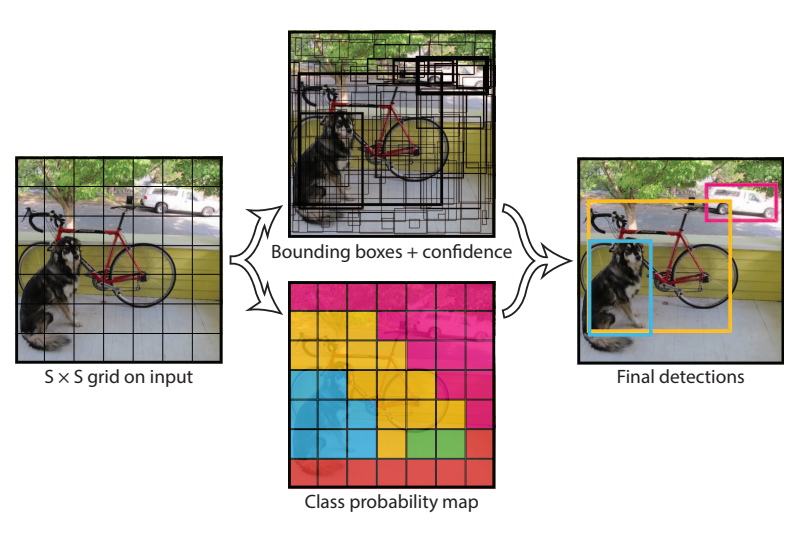
\includegraphics[height=6cm]{images/yolo.png} %
	\caption{\textit{YOLO} modelis \cite{redmon2016you}}%
	\label{fig:example}%
\end{figure}

Katrs ierobežojošais logs satur piecas prognozes: koordinātes, kas norāda loga centru attiecībā pret režģa šūnām, loga augstuma un platuma vērtības un pārliecības vērtību. Katra šūna prognozē nosacītās klašu varbūtības. Neatkarīgi no atrasto ierobežojošo logu skaita, katrai šūnai tiks piešķirta tikai viena klase.

Pētījumā \cite{redmon2016you} minētajai standarta \textit{YOLO} sistēmai ir 24 konvolūcijas slāņi, kam seko 2 pilnīgi savienotie slāņi. Pirmie konvolūcijas slāņi iegūst attēlu īpašības, kamēr pilnīgi savienotie slāņi prognozē objektu varbūtības un koordinātes.

\begin{figure}[h]%
	\centering
	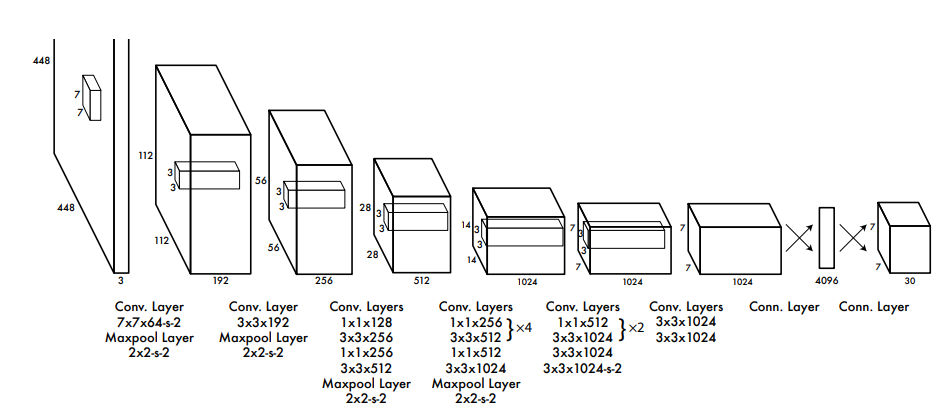
\includegraphics[height=7cm]{images/yoloarch.png} %
	\caption{\textit{YOLO} tīkla arhitektūra \cite{redmon2016you}}%
	\label{fig:example}%
\end{figure}
\newpage
Lai gan \textit{YOLO} ir labs un ātrs risinājums objektu detektēšanā, tam ir savi ierobežojumi:
\begin{itemize}
	\item Šī sistēma uzliek telpiskus limitus ierobežojošo logu prognozēm, jo katra režģa šūna prognozē tikai divus logus un katrai šūnai var piešķirt tikai vienu klasi. Šāds telpisks ierobežojums, limitē cik tuvumā esošus objektus \textit{YOLO} modelis var atrast. Tas nozīmē, ka sistēmai problēmas sagādā mazi objekti, kas atrodas grupās, piemēram, putni.
	\item Līdzīgi kā citas objektu detektēšanas metodes, \textit{YOLO} iemācās veikt ierobežojošo logu prognozes balstoties uz apmācības datiem, kas nozīmē, ja objektu detektēšana jāveic attēliem ar neierastiem izmēriem vai uzstādījumiem, \textit{YOLO} var būt grūti izšķirt objektus šajos attēlos.
	\item Attēlā 2.2 ir redzams, ka tīkla arhitektūrā ir vairāki apvienošanas slāņi (\textit{Maxpool layer}), kas nozīmē, ka ierobežojošo logu prognozēšanā tiek izmantotas salīdzinoši zemas kvalitātes (no angļu val. \textit{coarse}) īpašības. 
	\item Apmācības laikā izmantotā \textit{loss} funkcija pieņem, ka kļūdas mazajos ierobežojošajos logos ir tik pat būtiskas kā kļūdas lielajos logos, kas nav labs risinājums. Mazai kļūdai lielā logā ir maza ietekme, taču tikpat mazai kļūdai mazā logā var būt liela ietekme uz pārliecības rezultātiem. 
\end{itemize}   

\subsubsection{Faster-RCNN (\textit{Faster Region-Based Convolutional Neural Network})}
\textit{Faster-RCNN} ir objektu detektēšanas sistēma, kas sastāv no diviem tīkliem: reģionu noteikšanas tīkla (no angļu val. \textit{region proposal network}) jeb RPN, kas veido reģionu priekšlikumus, un no tīkla, kas šiem reģioniem veic objektu detektēšanu. RPN atgriež vairākus logus jeb priekšlikumus, kurus novērtēs klasifikators un regresors, lai noteiktu objektu esamību konkrētajā logā.

\begin{figure}[h]%
	\centering
	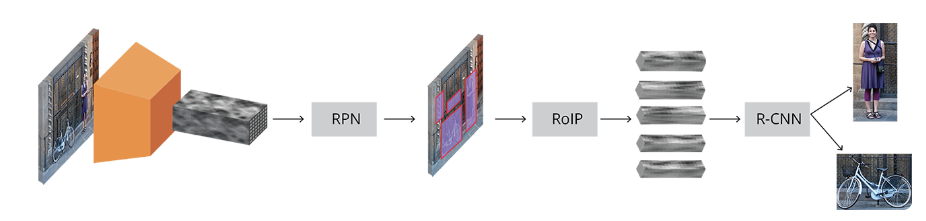
\includegraphics[height=3.5cm]{images/fastercnnarch.png} %
	\caption{\textit{Faster R-CNN} arhitektūra \cite{fasterrcnn}}%
	\label{fig:example}%
\end{figure}
\textit{Faster R-CNN} sistēmai ir salīdzinoši sarežģīta arhitektūra. Neiedziļinoties sīkumos, šī modeļa arhitektūra (attēls 2.3) sākas ar attēlu no kura ir nepieciešams iegūt: sarakstu ar ierobežojošajiem logiem, katram loga marķējumu (klases nosaukums) un katra marķējuma un ierobežojošā loga varbūtību. 

Ievades attēls ir vairākdimensiju masīvs, kuru padod ievadē konvolūcijas neironu tīklam līdz tiek iegūta īpašību karte. Pēc īpašību kartes iegūšanas, tā tiek nodota RPN. Izmantojot šīs īpašības, tīkls meklē iepriekš definētu skaitu ar reģioniem (ierobežojošajiem logiem, kurus sauc par \textit{anchors}), kuri var saturēt objektus (RPN nav svarīgi noskaidrot kādas klases objekts atrasts, tikai vai reģionā ir kāds objekts vai reģions satur tikai fona informāciju).  Šie reģionu logi ir fiksēta izmēra ierobežojošie logi, kuri ir vienmērīgi izvietoti attēla robežās. Pēc tam kad iegūts saraksts ar iespējamiem objektiem un to atrašanās vietām attēlā, detektēšanas problēma paliek krietni vienkāršāka. Izmantojot no konvolūcijas neironu tīkla iegūtās īpašību kartes un reģionu logus ar atbilstošajiem objektiem, pielieto RoI (no angļu val. Region of Interest) apvienošanu.
\begin{figure}[h]%
	\centering
	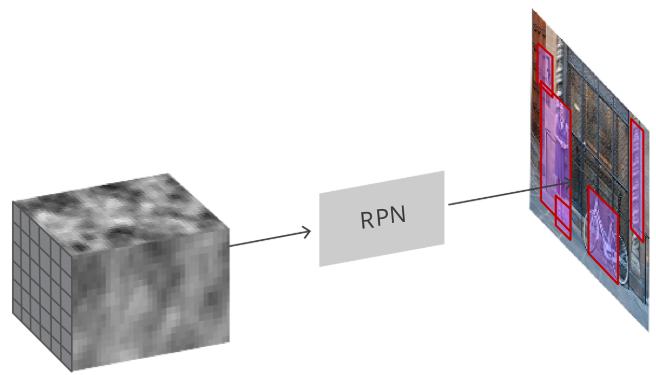
\includegraphics[height=5cm]{images/rpnstep.png} %
	\caption{RPN arhitektūra. RPN ievadē saņem no CNN atgriezto īpašību karti un attēlā ģenerē reģionu priekšlikumus. \cite{rpnarch}}%
	\label{fig:example}%
\end{figure}
Pēc RPN soļa ir iegūti vairāki prognozētie objekti, taču nav zināms kāda ir šo objektu klase. Vienkāršākais veids kā katram reģionam atrast klasi ir, samazināt šo reģionu un padot apmācītam tīklam, kas izmantojot iepriekš iegūtās attēla īpašības varēs risināt klasifikācijas problēmu, taču šāds risinājums nav efektīvs. Lai veiktu šāda veida klasifikāciju 1000 priekšlikumiem, tiks patērēts daudz laika un skaitļošanas resursu. Šo problēmu, \textit{Faster R-CNN} izstrādātāji risina vai vismaz samazina, izmantojot RoI apvienošanu \cite{roipooling}, ņemot iepriekš iegūto īpašību karti un iegūtos reģionus. 

Pēc RoI apvienošanas soļa seko R-CNN daļa, kas klasificē reģionu logu saturu vai arī atmet to, norādot reģiona marķējumā, ka tas ir fons. Kā arī R-CNN tīkls atjauno reģionu ierobežojošo logu koordinātes, lai ierobežojošais logs precīzāk pārklātu objektu. R-CNN izmanto katra piedāvātā reģiona īpašību karti, saplacina (no angļu val. \textit{flattens}) to un izmanto divus pilnīgās savienošanas slāņus ar ReLU kā aktivizācijas funkciju un atgriež objekta varbūtību un atjaunotā ierobežojošā loga robežas.

\begin{figure}[h]%
	\centering
	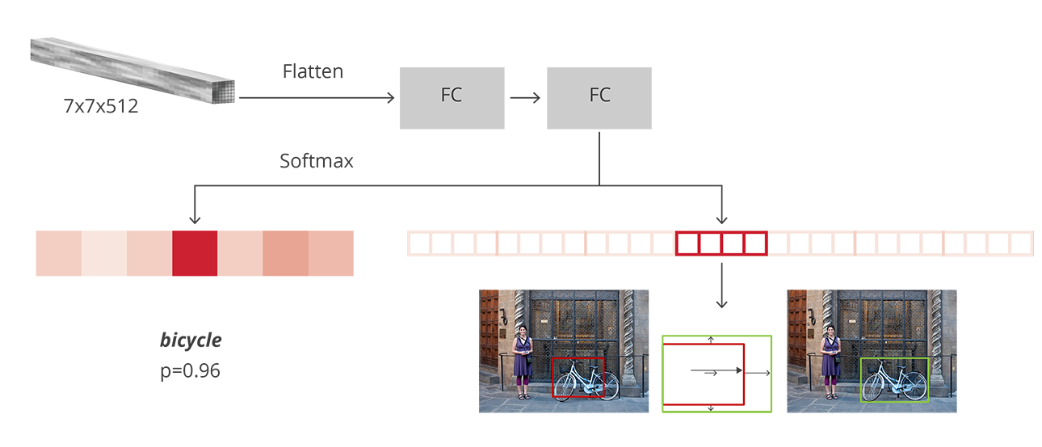
\includegraphics[height=5cm]{images/rcnnarch.png} %
	\caption{R-CNN arhitektūra \cite{fasterrcnn}}%
	\label{fig:example}%
\end{figure}

Līdzīgi kā pēc RPN soļa, pēc R-CNN soļa ir iegūti objekti, kuriem ir atrastas klases un kurus ir nepieciešams papildus apstrādāt. Lai  katram reģionam pielietotu ierobežojošo logu labojumus, tiek ņemts vērā kuras klases atrastā varbūtība bija ar visaugstāko vērtību (ja reģiona augstākā varbūtība ir klase "fons", tad šis reģions tiek ignorēts). Pēc gala objektu iegūšanas un "fona" objektu atmešanas, tiek pielietots uz klasēm balstīts NMS (\textit{non-maximum suppression}), lai novērstu vienas un tās pašas objekta instances detektēšanu vairākos reģionos \cite{hosang2017learning}.

\subsubsection{SSD (\textit{Single Shot MultiBox Detector})}

Īsumā, \textit{SSD} galvenā ideja ir tāda, ka tiek izmantots tikai viens neironu tīkls, kas padara risinājumu ātru un nav nepieciešamība pēc reģionu priekšlikumiem. Tā vietā, tiek izmantotas dažādi ierobežojošie logi, kuri tiek mainīti prognožu izdarīšanas laikā. Pētījums par \textit{SSD} kļuva pieejams 2016. gadā \cite{liu2016ssd} un šī detektēšanas sistēma uzstādīja jaunus rekordus veiktspējā un precizitātē objektu detektēšanas uzdevumu veikšanai. Lai labāk saprastu \textit{SSD} ir vērtīgi izskaidrot šīs sistēmas pilno nosaukumu:
\begin{itemize}
	\item \textit{\textbf{Single Shot}} : tas nozīmē, ka objektu lokalizācijas un klasifikācijas uzdevumus tiek veikts neironu tīkla slāņiem izejot cauri vienu reizi;
	\item \textit{\textbf{MultiBox}} : ir ierobežojošo logu regresijas tehnika, kuru izveidoja pētnieki, kas strādāja ar pie \textit{SSD} izveides;
	\item  \textit{\textbf{Detector}} : \textit{SSD} sistēmā neironu tīkls ir objektu detektors, kas arī klasificē detektētos objektus;
\end{itemize}
\newpage
\begin{figure}[h]%
	\centering
	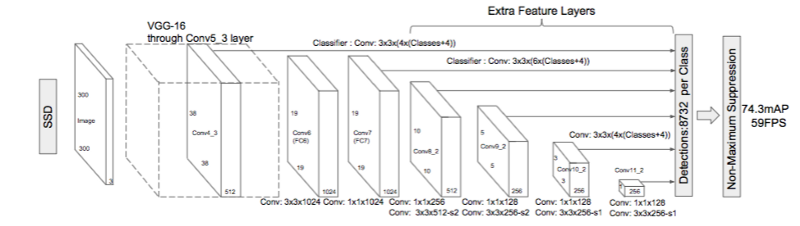
\includegraphics[height=4.5cm]{images/ssdarch.png} %
	\caption{SSD arhitektūra \cite{ssdarch}}%
	\label{fig:example}%
\end{figure}

Attēlā 2.6 ir attēlota \textit{SSD} arhitektūra, kur parādīts, ka šī objektu detektēšanas sistēma ir balstīta uz \textit{VGG Net} arhitektūru, taču netiek izmantoti standarta arhitektūras pilnīgi savienotie slāņi. \textit{VGG Net} neironu tīkla arhitektūra tiek izmantota kā \textit{SSD} bāze, jo tā darbojas ar augstu veiktspēju attēlu klasifikācijas uzdevumu veikšanā \cite{simonyan2014very}. Tai vietā, lai \textit{SSD} izmantotu pilnīgi savienotos slāņus no standarta \textit{VGG Net} konfigurācijas, tiek izmantoti papildus konvolūcijas slāņi, lai būtu iespējams iegūt attēla īpašības dažādos attēla izmēros un samazinātu katra nākamā slāņa ievadē saņemto attēlu izmēru. 

\textit{MultiBox} ir ierobežojošo logu regresijas metode, kas balstīta uz \textit{SSD} izstrādātāju pētījumu par objektu ierobežojošo logu koordināšu priekšlikumiem \cite{szegedy2014scalable}, kur nav zināmas objektu klases. \textit{MultiBox} \textit{loss} funkcija apvieno divas objektu detektēšanas mērvienības: \textit{confidence loss} un \textit{location loss}. \textit{Confidence loss} mēra, cik pārliecināts ir tīkls, ka aprēķinātais ierobežojošais logs satur objektu. \textit{Location loss} mēra cik tālu no tīkla prognozētajiem ierobežojošajiem logiem atrodas \textit{ground-truth} ierobežojošie logi apmācības datos. \textit{MultiBox loss} aprēķina sekojoši:

\begin{equation*}
\var{multibox_loss}
= \var{confidence_loss}
+ \var{alpha}
* \var{location_loss}
\end{equation*}
\textit{Alpha} minētajā vienādojumā palīdz balansēt \textit{location loss} vērtību. Līdzīgi kā citām dziļās mašīnmācīšanās sistēmām, ir nepieciešams atrast vienādojuma parametrus, kas vislabāk samazina \textit{loss} funkciju, tādējādi pietuvinot tīkla prognozes \textit{ground-truth} vērtībām.

\textit{MultiBox} pētnieki veidojot šo metodi ieviesa jaunu terminu \textit{priors}. \textit{Priors} ir iepriekš aprēķināti, fiksēta izmēra ierobežojošie logi (\textit{Faster R-CNN} sistēmā šos logus sauc par \textit{anchors}), kas cieši sakrīt ar \textit{ground-truth} ierobežojošo logu izvietojumu. Balstoties uz šiem iepriekš aprēķinātajiem ierobežojošiem logiem, \textit{MultiBox} tos izmanto kā prognozes un mēģina regresēt tuvāk \textit{ground-truth} ierobežojošajiem logiem. Beigās \textit{MultiBox} saglabā tikai labākās prognozes ar minimizētām \textit{location loss} un \textit{confidence loss}. 

\textit{SSD} pētījumā ir veikti uzlabojumi standarta \textit{MultiBox} sistēmai, kas padara šo objektu detektēšanas sistēmu vēl spējīgāku lokalizēt un klasificēt objektus. \textit{SSD} katra īpašību kartes šūna ir savienota ar dažādu izmēru un dažādu proporciju ierobežojošajiem logiem (\textit{priors}). Šie logi ir manuāli izvēlēti, kas, teorētiski, ļauj \textit{SSD} darboties ar dažādi konfigurētiem ievades datiem. Pieņemot, ka ir definēts \textit{c} skaits klašu, katrai īpašību kartes šūnai ir definēts \textit{b} skaits ierobežojošo logu un īpašību kartes izmērs ir \textit{f}, \textit{SSD} aprēķinātu \textit{f * b * (4 + c)}
vērtības šai īpašību kartei. 

\begin{figure}[!htb]
	\minipage{0.32\textwidth}
	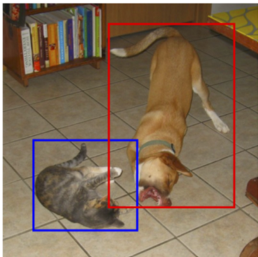
\includegraphics[width=\linewidth]{images/ssdgtboxes.png}
	\caption{Attēls ar \textit{ground-truth} logiem \cite{liu2016ssd}}
	\endminipage\hfill
	\minipage{0.32\textwidth}
	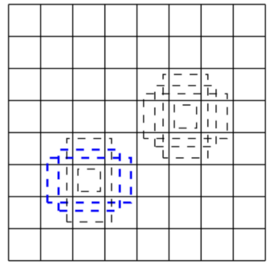
\includegraphics[width=\linewidth]{images/ssd88featmap.png}
	\caption{8 x 8 izmēra īpašību karte \cite{liu2016ssd}}
	\endminipage\hfill
	\minipage{0.32\textwidth}%
	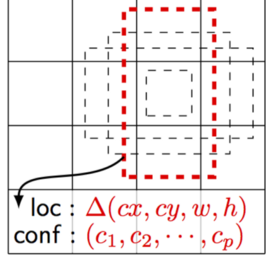
\includegraphics[width=\linewidth]{images/ssd44featmap.png}
	\caption{4 x 4 izmēra īpašību karte \cite{liu2016ssd}}
	\endminipage
\end{figure}

Attēlā 2.7 ir parādīts, ka apmācības laikā \textit{SSD} ir tikai nepieciešams ievades attēls un \textit{ground-truth} logi, kas atspoguļo objektus attēlā. Izmantojot konvolūcijas principus, tiek novērtēti daži ierobežojošie logi, dažādos attēla mērogos un tie tiek uzglabāti īpašību kartēs ar dažādiem izmēriem (attēlā 2.8 ir parādīta 8x8 izmēra īpašību karte un attēlā 2.9 4x4 izmēra īpašību karte). Katram logam aprēķina formas nobīdi no patiesās un pārliecības vērtības katrai objektu kategorijai (attēlā 2.9 c1,c2,...,cp). Apmācības laikā, definētie logi tiek pieskaņoti \textit{ground-truth} logiem. Piemēram, attēlā 2.7 parādīts, ka divi ierobežojošie logi ir pieskaņoti kaķim un sunim. Modeļa \textit{loss} (modeļa kopējā precizitāte ņemot vērā apmācības un validācijas datus) ir svērtā summa starp \textit{localization loss} un \textit{confidence loss}. 

Līdzīgi \textit{Faster-RCNN}, arī \textit{SSD} kā vienu no pēdējiem soļiem tīkla izpildes laikā izmanto \textit{non-maximum suppression} (NMS). Pēc detektēšanas soļa iegūtie logi tiek šķiroti pēc norādīta sliekšņa, kas atkarīgs no \textit{confidence loss} vērtības. Tikai labākos logus saglabā un pārējie (mazāks \textit{confidence loss} par sliekšņa vērtību) tiek atmesti. NMS pielietošana nodrošina, ka tikai labākās logu prognozes tīkls saglabās un trokšņainās atmetīs.
 \newpage
\begin{figure}[h]%
	\centering
	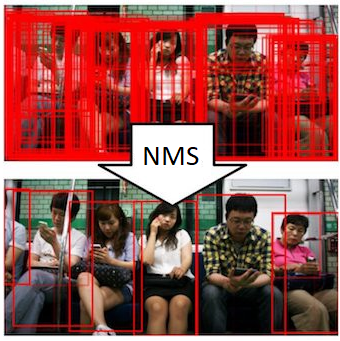
\includegraphics[height=4cm]{images/nms.png} %
	\caption{\textit{Non-maximum supression} piemērs \cite{liu2016ssd}}%
	\label{fig:example}%
\end{figure}

\textit{SSD} pētījumā \cite{liu2016ssd} ir aprakstīti novērojumi par sistēmas darbību:
\begin{itemize}
	\item Jo vairāk iepriekš definētie logi, jo precīzāk notiek detektēšana, taču tas negatīvi ietekmē sistēmas ātrumu;
	\item Izmantojot \textit{MultiBox} vairākos slāņos, sistēma objektu detektēšanu veic precīzāk, jo detektors tad darbojas ar dažādu izšķirtspēju īpašībām;
	\item \textit{SSD} mēdz jaukt objektus, kam ir līdzīgas klases (piemēram, dzīvnieki ar 4 kājām);
	\item \textit{SSD} vāji strādā ar maziem objektiem, jo tie var neuzrādīties visās īpašību kartēs. Palielinot ievades attēlu izšķirtspēju ir iespējams samazināt šo problēmu.
\end{itemize}

Ņemot vērā tikai pētījumos \cite{redmon2016you,ren2015faster,liu2016ssd} pieejamo informāciju, dotajā brīdī, \textit{Faster R-CNN} ir labākā objektu detektēšanas sistēma, ja vērā ņem tikai precizitātes vērtējumus un lietotājam ir pieejami neierobežoti skaitļošanas resursi. Ja lietotājiem ir ierobežoti skaitļošanas resursi, \textit{SSD} ir labākais ātruma un precizitātes kompromiss. Ja par precizitāti nav jāuztraucas, bet ir vēlme pēc ļoti ātras sistēmas, tad labākais variants ir \textit{YOLO}. Lai gan \textit{Faster R-CNN} labāk par pārējiem spēj atrast maza izmēra objektus, sistēma ir lēna un nenodrošina reālā laika detektēšanu. Gan \textit{YOLO}, gan \textit{SSD} sistēmas nodrošina reālā laika objektu detektēšanu, kas ir nepieciešams šī darba ietvaros. Ņemot vērā augstāk minēto informāciju, pētījuma ietvaros radītais risinājums izmantos \textit{SSD} objektu detektēšanas sistēmu, jo tā ir labākā precizitātes un ātruma apvienojums un apmācību ir iespējams veikt ar lietotājiem pieejamākām ierīcēm. 

Pēc objektu detektēšanas metodes izvēlēšanās, šī pētījuma ietvaros ir nepieciešams apskatīt sekošanas risinājumus, kuru izmantot gala risinājumā. Lai veiksmīgi veiktu cilvēku plūsmas analīzi, ar izvēlēto objektu detektēšanas metodi vien nepietiek, objektiem ir arī jāseko. Šādā risinājumā ir vērtīgi ieviest sekošanas risinājumu sekojošu iemeslu dēļ:
\begin{itemize}
	\item Sekošanas algoritmi darbojas ātrāk kā detektēšanas algoritmi. Šādu argumentu var izskaidrot ar to, ka sekojot objektam, kas jau ir atrasts iepriekšējā kadrā, sistēmai ir pieejama informācija par objekta attēlojumu, atrašanās vietu, kustības virzienu un kustības ātrumu. Sekošanas algoritms izmantos visu šo informāciju, lai nepazaudētu objekta atrašanās vietu, kamēr objektu detektēšanas algoritmam katrs katrs ir jāapstrādā no jauna.
	\item Sekošanas algoritmi ir kā drošības tīkls gadījumā, ja detektēšanas risinājumi vairs nevar atrast kādu no iepriekšējos kadros noteiktajiem objektiem. Piemēram, ja starp objektu un video kameru nostājas šķērslis, tas detektēšanas risinājumiem sagādās pamatīgas problēmas, kamēr labs sekošanas risinājums nepazaudētu objekta atrašanās vietu.
	\item Sekošanas algoritmi veido savienojumus starp video kadriem, tādā veidā saglabājot objekta identitāti.
\end{itemize}

Sekošanas mērķis ir atrast objektu dotajā video kadrā, pieņemot, ka objektam ir veiksmīgi sekots visos iepriekšējos kadros vai dotajā kadrā pirmo reizi atrasta šī objekta instance. Tā kā objektam ir sekots līdz dotajam kadram, ir zināms, ka objekts kustas, kas nozīmē, ka ir zināmi kustības modeļa parametri. Kustības modeli veido iepriekšējos kadros noteiktā objekta atrašanās vieta un ātrums. Nezinot neko citu kā kustības modeļa parametrus jau ir iespējams izteikt diezgan precīzu minējumu kur dotajā kadrā varētu atrasties objekts. Risinot sekošanas problēmu video fragmentos, ir pieejama informācija par vairāk kā tikai objekta kustību ir zināms arī objekta izskats visos iepriekšējos kadros. Zinot objekta izskatu, ir iespējams veidot izskata modeli, šādu modeli var izmantot, lai precizētu objekta atrašanās vietu pēc tam, kad balstoties uz kustības modeli ir izdarīts minējums par aptuveno objekta atrašanās vietu. Ja objekts ir vienkāršs un starp kadriem izskatu nav mainījis, tad izskata modeli var izmantot kā veidni, kuru meklēt jaunajā kadrā. Diemžēl, objekta izskats var pamatīgi mainīties, lai cīnītos ar šo problēmu modernie sekošanas risinājumi izmanto izskata modeli kā klasifikatoru, kurš tiek apmācīts algoritma izpildes laikā. 

Gala risinājuma izstrādes laikā tika apskatīti \textit{OpenCV} programmatūrā piedāvātie sekošanas algoritmi: \textit{Multiple Instance Learning} (MIL) un \textit{AdaBoost} kā arī \textit{SiamFC} sekošanas algoritms, kas neietilpst \textit{OpenCV} bibliotēkā, bet ir aprakstīts Luka Bertinetto pētījumā \cite{bertinetto2016fully}.

\subsubsection{Multiple Instance Learning}

\subsubsection{AdaBoost}
\subsubsection{SiamFC}

%% Nenumurēta nodaļa, kas uzrādās satura rādītājā
\chapter*{Secinājumi un priekšlikumi}
\addcontentsline{toc}{chapter}{Secinājumi un priekšlikumi}
\begin{enumerate}
\item \textbf{Secinājumi un priekšlikumi} jāraksta tēžu veidā.
\item Secinājumiem jāatspoguļo svarīgākās atziņas, kas izriet no pētījuma, satur atbildes uz ievadā izvirzīto mērķi un uzdevumiem.
\item Secinājumos jāpaskaidro veiktā pētījuma tautsaimnieciskā, zinātniskā vai praktiskā nozīme un autora personīgais veikums uzdevuma risināšanā.
\item Secinājumus nedrīkst pamatot ar datiem un faktiem, kas nav minēti darbā.
\item Secinājumos nav pieļaujami citāti no citu autoru darbiem, tajos jāatspoguļo tikai darba autora domas, spriedumi, atziņas.
\item Priekšlikumiem jāizriet no darbā veiktajiem pētījumiem un izdarītajiem secinājumiem, tiem jābūt konkrētiem un pamatotiem.
\item Priekšlikumos apkopo arī darbā pamatotās rekomendācijas trūkumu novēršanai.
\item Secinājumi un priekšlikumi jānumurē ar arābu cipariem.
\end{enumerate}
 %% Ērtāk visu failā secinajumi-un-priesklikumi.tex

\bibliographystyle{unsrt}
\selectlanguage{latvian}
\bibliography{src/links,src/articles,src/books}	%to load the *.bib files ../articles,../books,
\addcontentsline{toc}{chapter}{Izmantotās literatūras un avotu saraksts}


\chapter*{Galvojums}
\addcontentsline{toc}{chapter}{Galvojums}
 Ar šo es, \defAutors, galvoju, ka maģistra darbs ir izpildīts patstāvīgi un bez citu palīdzības. No svešiem pirmavotiem ņemtie dati un definējumi ir uzrādīti darbā. Šis darbs tādā vai citādā veidā nav nekad iesniegts nevienai citai pārbaudījumu komisijai un nav nekur publicēts.

\vspace{1in}
\defGads.gada \rule{1cm}{0.2pt}.\rule{3cm}{0.2pt}
\label{LastPage}

%% Te vajadzētu pielikumus
\appendix
\chapter{Pirmais pielikums}

\addtocounter{nofappendices}{1}
\label{appendix:tituldati}
%\lstinputlisting[firstline=6, lastline=15]{../codes/calcHomogInfModel.m}
\lstinputlisting[firstline=18, lastline=25]{README.md}

\chapter{Otrais pielikums}

\addtocounter{nofappendices}{1}
\label{appendix:tituldati2}
\lstinputlisting{README.md}

%% Vēl jāpievieno atzīmes lapa
\pagebreak
%% Šai lapai nevajag numerāciju
\pagestyle{empty}
\begin{center}
 Maģistra darbs aizstāvēts Valsts pārbaudījumu komisijas sēdē\\
 \vspace{1em}
\end{center}
\defGads.gada \rule{1cm}{0.2pt} . \rule{3cm}{0.2pt}\\\\
un novērtēts ar atzīmi \rule{4cm}{0.2pt} \\\\\\
Protokols Nr. \rule{1cm}{0.2pt}\\\\\\
Valsts pārbaudījumu komisijas \\\\
priekšsēdētājs \rule{7cm}{0.2pt}.\\
\hspace*{5cm}\textit{\raisebox{1em}{paraksts}}


\end{document}
